\documentclass[letterpaper]{article}


\PassOptionsToPackage{numbers}{natbib}
\usepackage[preprint]{neurips_2023}
\usepackage[utf8]{inputenc} % allow utf-8 input
\usepackage[T1]{fontenc}    % use 8-bit T1 fonts
\usepackage{hyperref}       % hyperlinks
\usepackage{url}            % simple URL typesetting
\usepackage{booktabs}       % professional-quality tables
\usepackage{amsfonts}       % blackboard math symbols
\usepackage{nicefrac}       % compact symbols for 1/2, etc.
\usepackage{microtype}      % microtypography
\usepackage{xcolor}         % colors
\usepackage{tikz}
\usepackage{pgfplots}
\usepackage{tabularx,ragged2e}
\usepackage{amsmath}



\newcolumntype{L}{>{\RaggedRight}X}
\pgfplotsset{width=10cm,compat=1.9}


%%%%%%%%%%%%%%%%%%%%%%%%%%%%%%%%%%%%%%%%%%%%%%%%%%%%%%%%%%%%


\title{Generalizable IC Routing using Deep RL with a GNN-based Policy Network}

\author{%
    Roozmehr Jalilian, Shidi Xi \\
    Department of Electrical \& Computer Engineering \\
    The University of British Columbia \\
    \texttt{\{roozmehr.jalilian,xsd99\}@ece.ubc.ca} \\
    Vancouver, BC V6T 1Z4
}


\begin{document}


\maketitle


\begin{abstract}
Routing in integrated circuits (IC) design is often modeled as a pathfinding problem and has consistently represented one of the most challenging aspects due to its complexity and time-consuming nature. Even with state-of-the-art commercial CAD tools, routing complex designs can take hours, if not days. Consequently, there is a growing interest in applying machine learning-based approaches to overcome these challenges. In previous work, we introduced a novel reinforcement learning (RL) approach for routing. While this RL router outperformed the baseline, it was limited by poor generalizability, requiring a new policy to be trained from scratch for each problem. In this project, we aim to address this limitation by introducing a novel graph neural network (GNN) as the policy network for the RL router. This enhancement allows the agents to generalize their learned routing policies to new, unseen designs, reducing the computation time significantly.
%TODO: Briefly mention the results that we've obtained (if it helps, that is!).
\end{abstract}

\section{Introduction}
Physical design is a crucial phase in the IC design process, wherein the logical representation of the chip is converted into a physical geometric layout essential for fabrication foundries. This stage is subdivided, with routing being a key step were pins specified by netlists are connected using wires and vias. The quality of the routing, often evaluated by wirelength and egde overflow, impacts vital chip metrics like performance, power, and area \cite{Hu2001}.

For 2-dimensional circuit layouts, routing can be modeled as a pathfinding problem in a 2D grid, were the objective is to establish paths connecting pins placed on different coordinates of the said grid. This grid can be treated like a graph, with the circuit's pins placed on its nodes and the connections between them occupying its edges. Each edge possesses a capacity feature, indicating the maximum number of permissible wires due to the physical constraints of wire thickness and finite space within a chip region. An optimal routing solution seeks to minimize total wire length and avoid edge overflow (usage of an edge exceeding its capacity), ensuring all connections are efficient and within capacity.

Two important terminologies here are net and netlist. A {\it net} refers to a set of pins requiring connection, and a {\it netlist} is a set consisting of multiple nets that need routing during the process. For clarity, we will use the terms {nodes} and {pins} interchangeably throughout this paper.

Traditional routing often involves decomposing multi-pin nets into 2-pin sub-nets, sequentially routed using maze-routing algorithms like A*. Decomposition typically involves constructing a minimum spanning tree from the pins. Despite the simplicity and efficacy of this approach, the net-ordering issue persists: later routed nets face blockages leading to edge overflow, while early-stage nets lack foresight to conserve resources for subsequent nets. Designers typically resort to rip-up and re-route strategies, were congested pathways are removed and re-routed.

Complexities of the traditional routing algorithms have inspired researchers to use machine-learning-based techniques instead. One such technique is reinforcement learning (RL), and specifically, its deep variant (DRL), which is a fusion of RL and deep neural networks. It has showcased capabilities exceeding human performance in various contexts \cite{mnih2013playing}.

In prior research, we introduced a multi-agent RL router to address the IC routing challenge. Each agent, tasked with routing one individual net, operated concurrently under a shared super policy, as we designed the agents to be homogeneous and fully-cooperative. Trained with proximal policy optimization (PPO) \cite{Schulman2017} and evaluated against benchmarks, this RL router demonstrated superior performance compared to the A* baseline. However, a limitation emerged: the policy, though effective for specific benchmarks, lacked generalizability for other, albeit similar, problems. We attributed this shortfall to the policy neural network's architecture, comprising several fully connected (FC) layers, which struggled to extract rich information from the state encodings.

Contrastingly, graph neural networks (GNNs) exhibit robust generalization capabilities when processing graphical data \cite{Almasan2022,Wang2018}, aligning with the routing problem’s grid graph model. In this project, we introduce a novel message-passing GNN architecture integrated into the RL router’s policy network. The GNN accepts the routing grid graph from the environment as state input and determines actions accordingly. This innovation aims to bolster the RL router’s ability to generalize trained policy to problems not encountered during training, promising substantial reductions in computation time.


\section{Related work}
Numerous studies in existing literature have verified the effectiveness of employing Graph Neural Networks (GNNs) within the policy/value network of Reinforcement Learning (RL) models to enhance generalization, especially when the agent’s environment is graph-representable. However, to our knowledge, no existing study has directly explored the use of GNN equipped RL for IC routing.

\cite{Liao2020} introduced an RL IC router trained via a Deep Q-Network (DQN), utilizing a multi-layer perceptron (MLP) as the RL agent's value network. However, similar to our previous work, it showed a lack of generalization. Contrastingly, \cite{Almasan2022} incorporated a GNN as the value network of an RL agent, also trained by DQN. This approach manifested notable generalization capabilities in network routing—a field bearing similarities to IC routing—and serves as the principal inspiration for our current proposal. In parallel, both \cite{Chen2023} and \cite{Wang2018} echoed the integration of GNNs with RL models wherein the operational problems are graphs. Furthermore, \cite{Mirhoseini2021} and \cite{Yue2022} adopted GNNs as encoder layers for their respective RL policy and value networks.

    
\section{Methodology}

\subsection{IC routing as a pathfinding problem}
\autoref{fig:grid} illustrates a simplified IC routing problem, represented as a pathfinding problem on a grid graph. A net consists of two pins, (0,0) and (3,3), needs to be routed. Additionally, each edge has a capacity of 1. In other words, the task is to find a path with minimum length between these two points while every edge on the graph can at most be traversed once.

\begin{figure}[h!]
    \centering
    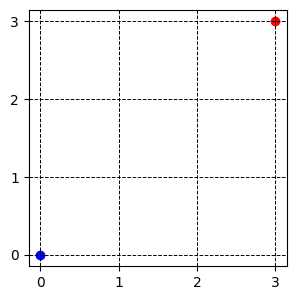
\includegraphics[width=0.3\textwidth]{figure/grid_grap.png}
    \caption{The grid graph of a simple IC routing problem.}
    \label{fig:grid}
\end{figure}

\subsection{GNN-based RL framework for IC routing}
An illustration of the proposed RL routing framework is shown in \autoref{fig:overview}. The framework consists of an agent repeatedly interacting with an environment. At time step $t$, the agent receives observation $S_{t}$ and reward $R_{t}$, and at the next time step, $t+1$, it provides action $A_{t+1}$ to the environment. The agent is governed by a policy and a value network. The policy network is a function approximator of the policy $\pi_{\theta_1}(a|s)=P(A_{t+1}=a|S_{t}=s)$, which represents the probability of taking action $a$ given the environment is in state $s$. This function is represented by our proposed GNN, parameterized by $\theta_1$, which will be described shortly. The value network is the approximator of the value function $V_{\theta_2}(s)$, which is used to update the parameters of the policy network $\theta_1$. It is represented by another GNN with the same architecture with the policy network. However, these two networks do not share parameters with each other, i.e., $\theta_1\neq\theta_2$. 
\begin{figure}[h!]
    \centering
    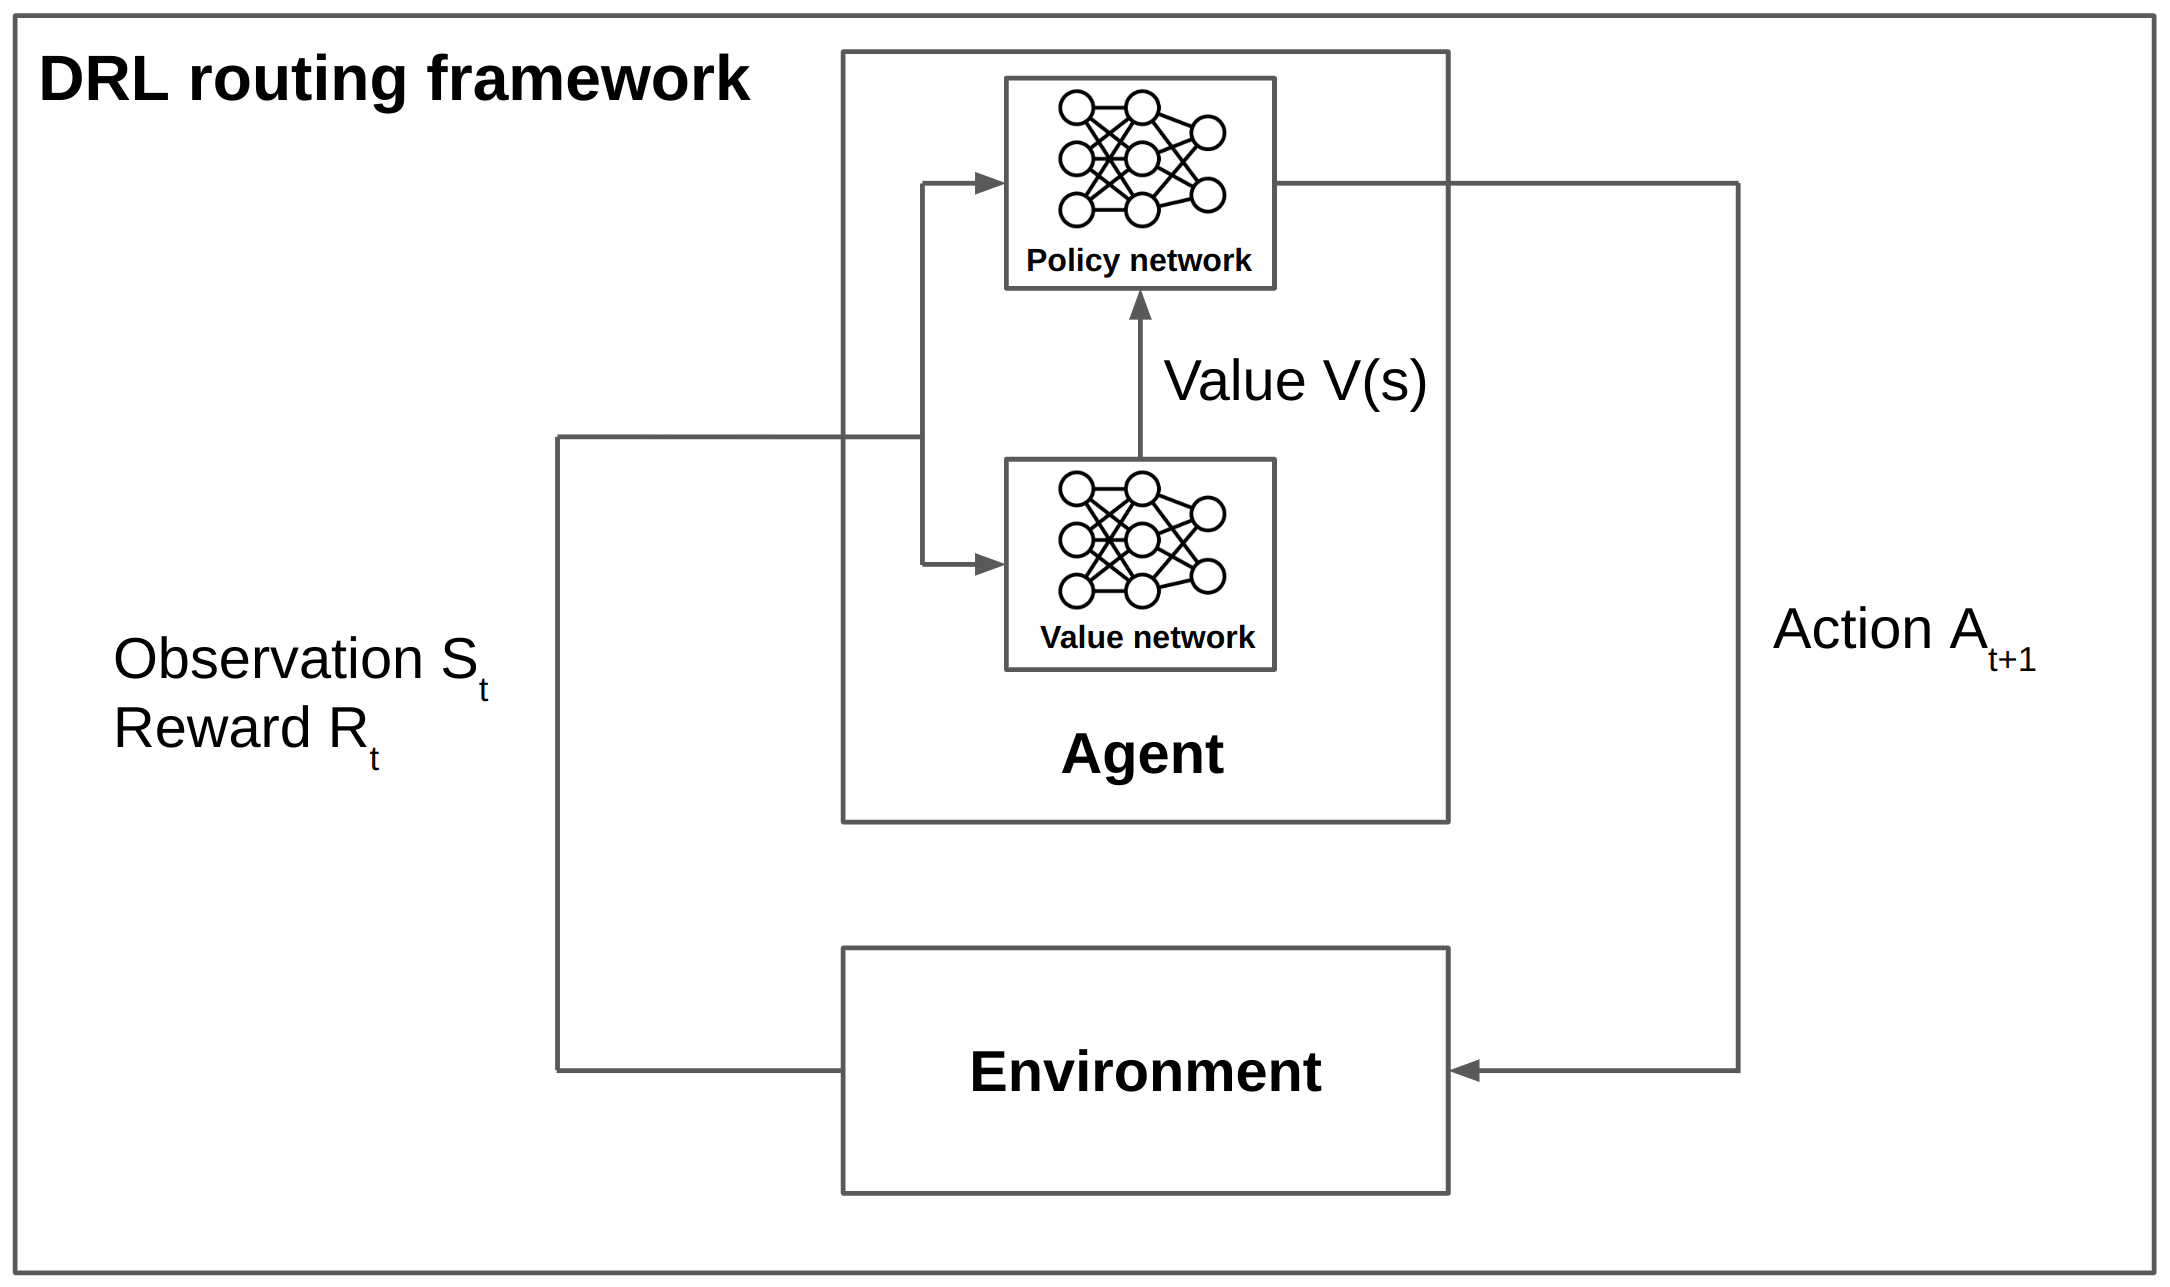
\includegraphics[width=\textwidth]{figure/overview.png}
    \caption{The overview of the proposed DRL routing framework.}
    \label{fig:overview}
\end{figure}

\subsection{Environment}
The environment represents the grid pathfinding problem. It receives actions from the agent, update internal states, and provide new observation state and reward to the agent.
\subsubsection{Observations}
Observations are the states that an agent can perceive from the environment, encapsulating crucial information about the environment itself. It consists of a node feature matrix $\mathbf{X} \in \mathbb{R}^{N \times 2}$, an edge feature matrix $\mathbf{E} \in \mathbb{R}^{N \times N}$, and an adjacency matrix $\mathbf{A} \in \mathbb{R}^{N \times N}$. In a grid consists of $N$ nodes, each node is denoted by a 2D feature vector $x$ with both elements being binary. The first element $x_1$ indicates the agent is currently at this node if it equals to 1, while $x_2$ indicates the target position. $\mathbf{E}$ contains the scalar capacity of each edge, which will be reduced by 1 each time the agent walks across a particular edge. 

%TODO: demonstration

\subsubsection{Reward function}
The environment imposes a -1 penalty on the agent for each step taken that does not lead to the target, fostering a drive to discover the shortest path. Reaching the target (the agent and the target sit at the same node) yields a +100 reward, and when this happens, there will be a vector $x$ in $\mathbf{X}$ having both of its two elements equal to 1.
\begin{equation}
    R(\mathbf{X}) = \begin{cases} 
    100 & \text{if } \exists i \in \{1, 2, \ldots, N\}, x_{i_1} = x_{i_2} = 1, \\
    -1 & \text{otherwise}.
    \end{cases}
    \end{equation}
This configuration incites the agent to minimize wirelength, equating to the distance traveled to reach the target. Unnecessary deviations culminate in diminished cumulative rewards.

\subsection{Agent}
The agent receives observations and rewards from the environment, which are fed into the policy and value network to generate probability distributions of actions. During training, the networks' parameters are tuned such that a sequence of actions leading to maximum cumulative reward will be generated. 

\subsubsection{Actions}
The actions are encoded by an integer ranges from 0 to 3, meaning the agent goes up, right, down, or left from its current position by traversing through a particular edge. After each action the agent has taken, the environment will transition into a new state, and $\mathbf{E}$ and $\mathbf{X}$ will be updated.

\subsubsection{GNN design}
The GNN takes $\mathbf{A}$, $\mathbf{E}$ and $\mathbf{X}$ as input, it first encode the node feature matrix $\mathbf{X}$ into hidden representation matrix $\mathbf{H^t}$. That is,
\begin{equation}
    h_i^0 = F_{encode}(x_i)
\end{equation}
with $F_{encode}$ being an MLP. The superscript $t$ of $H$ represents the number of message passing performed. Initially, when no message passing has been performed, $t=0$. 

The second step is to compute the message for each node, formulated as 
\begin{equation}
    m_{ji} = F_{message}([h_j^t, h_i^t, e_{ji}])
\end{equation}
with $F_{message}$ being another MLP. $[h_j^t, h_i^t, e_{ji}]$ represents the concatenation of $h_j^t$, $h_i^t$, and $e_{ji}$, where $h_j^t$ and $h_i^t$ are hidden states of node $i$ and $j$, extracted from $\mathbf{H^t}$. $e_{ji}\in \mathbf{E}$ is the scalar capacity of the edge connecting the two nodes. The third step is to aggregate the messages for each node from all of their neighboring nodes. 
\begin{equation}
    \bar{m}_{i} = \sum_{j\in N_{in}} m_{ji}
\end{equation}
The aggregated message $\bar{m}_{i}$ of node $i$ is the element-wise summation of messages sent towards node $i$ from all of its $N_{in}$ neighbors. The forth step updates the hidden states of all nodes using their current states and aggregated messages. 
\begin{equation}
    h_{i}^{t+1} = F_{update}(h_{i}^t, \bar{m}_{i})
\end{equation}
Here, $F_{update}$ is implemented by using a gated recurrent unit (GRU). The message passing, i.e., step 2 to 4, will be performed $T$ times, where $T$ is the diameter of the input grid graph. 

The final step is to read out the policy logits for the policy network, or the value for the value network. The policy logits will be further fed into a softmax layer to get the probability distribution of actions. This step sum all node states $h_i^T$ element-wisely, and forward the result to an MLP.
\subsection{Training}
The proposed GNN is integrated into our RL routing framework, serving as its policy and value network. The training will be conducted using PPO (REF) with RLlib. The GNN's parameters will be refined through stochastic gradient descent, guided by value feedback from the value network.

    
\section{Experiments}
We constructed an MLP-based RL framework as a baseline and we compared the performance of the GNN-based RL network with it. Both frameworks were trained in benchmark A, and the obtained policies were tested using benchmark B. The details of the two benchmarks are listed in the table below.

\begin{table}[h!]
    \caption{Two benchmarks used for training and testing.}
    \centering
    \begin{tabular}{|c c c|}
        \hline
        \hline
         & Benchmark A & Benchmark B \\
        \hline
        Length & 4 & 4 \\
        Width & 4 & 4 \\
        Source node coordinates & (0,0) & (3,0) \\
        Target node coordinates & (3,2) & (0,1) \\
        Edge capacity & 2 & 2 \\
        \hline
        \hline
    \end{tabular}
    \label{tab:benchmark}
    \end{table} 

\subsection{Comparing training efficiency}
This experiment aims to compare the training efficiency of the GNN-equipped router with the baseline router, both trained on the same benchmark. We will assess their performance by examining the plots of reward versus training iterations. The objective is to evaluate the training efficiency of the GNN-equipped router in comparison to the baseline. As suggested by \cite{Wang2018}, we anticipate that the new design will demonstrate comparable, if not superior, training efficiency.

\subsection{Comparing Zero-Shot Performance} \label{m:0}
We will employ the zero-shot policies derived from the previous experiment to perform inference on several unseen benchmarks. These benchmarks will feature netlists with canvas sizes, numbers of nets, and total numbers of pins per net that resemble the training benchmark. The comparison criteria will include rewards and routing solution quality (wire length, overflow). We predict that the new GNN-equipped design will surpass the baseline in performance.

THIS PART DIDN'T WORK OUT. BOTH GNN AND MLP GOT 0 REWARD. 

\subsection{Comparing Fine-Tuning Performance}
This experiment is designed to evaluate the scalability of the GNN to more complex problems. We will initiate zero-shot inference on benchmarks characterized by different numbers of nets, chip canvas sizes, and numbers of pins per net than the training benchmark. We anticipate a decrease in zero-shot performance compared to the results of \autoref{m:0}, indicating a likely need for policy fine-tuning.

Both the new design and baseline policies will undergo fine-tuning for an equal number of iterations. We will compare their performances based on rewards and solution quality metrics. Our expectation leans towards the new GNN-equipped design demonstrating superior adaptability and performance after fine-tuning.

THIS PART DIDN'T WORK OUT EITHER. BOTH GNN AND MLP SHOWED FIAT LINE.

\begin{figure}[h!]
    \centering
    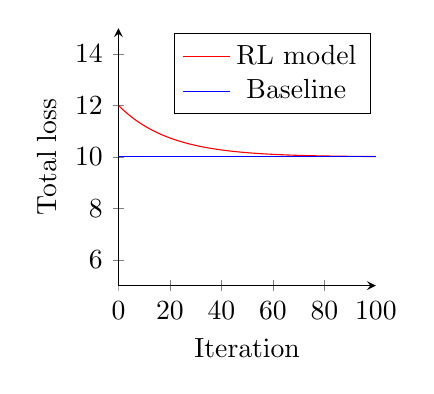
\begin{tikzpicture}
        \begin{axis}[
            width=0.4\textwidth,
            height=0.4\textwidth, 
            axis lines = left,
            xlabel = Iteration,
            ylabel = Total loss,
            ymin=5, ymax=15,
            ]
            % The reward function
            \addplot [
            domain=0:100, 
            samples=100, 
            color=red,
            ]
            {10 + 2 * exp(-x / 20)};
            \addlegendentry{RL model}
            % Baseline
            \addplot [
            domain=0:100, 
            samples=100, 
            color=blue,
            ]
            {10};
            \addlegendentry{Baseline}
        \end{axis}
    \end{tikzpicture}
    \caption{Placeholder figure for total loss vs. time. Not related to any aforementioned experiments.}
\end{figure}

\begin{table}[h!]
    \caption{Placeholder table for the experiments. Not related to any aforementioned experiments.}
    \centering
    \begin{tabularx}{\textwidth}{LLLLLLL}
        \toprule
        \multicolumn{4}{c}{Benchmark specs} &
        \multicolumn{3}{c}{Results} \\
        \cmidrule(r){1-4}
        \cmidrule(r){5-7}
        Name & Canvas size & \# of nets & Avg. \# of pins per net & Runtime (s) & Max. memory usage (MB) & Total wirelength \\
        \midrule
        test1 & \(8 \times 8\) & 5 & 2.5 & 1.25 & 250 & 100 \\
        test2 & \(6 \times 6\) & 3 & 1 & 0.60 & 150 & 70 \\
        \bottomrule
    \end{tabularx}
\end{table}
    
%%%%%%%%%%%%%%%%%%%%%%%%%%%%%%%%%%%%%%%%%%%%%%%%%%%%%%%%%%%%
    
{
\small
\bibliographystyle{IEEEtranN}
\bibliography{references}
}

%%%%%%%%%%%%%%%%%%%%%%%%%%%%%%%%%%%%%%%%%%%%%%%%%%%%%%%%%%%%


\end{document}